%!TEX root = ../dissertation.tex

\chapter{Experiment}
\label{chp:experiment}
%\epigraph{Las dein Auge am Rohr, Sagredo. Was du siehst, ist, dass es keinen Unterschied zwischen Himmel und Erde gibt. Heute ist der 10. Januar 1610. Die Menschheit trägt in ihr Journal ein: Himmel abgeschafft.}{Bertolt Brecht, Leben des Galilei}

\epigraph{Keep your eye at the telescope, Sagredo. What you see means that there is no difference between Heaven
and Earth. Today is the 10th January 1610. Mankind will write in its journal: Heaven abolished}{Bertolt Brecht, \textit{Life of Galileo}}
\section{The Large Hadron Collider}
The Large Hadron Collider (LHC) is a 27 km long circular accelerator, positioned at CERN, the European Organization for Nuclear Research, on the Swiss-French border. Constructed approximately 100 to 150 metres underground, LHC has established itself as the world's largest and most powerful particle accelerator, capable of propelling protons and heavy ions to unprecedented energies.

Before reaching the LHC, protons are extracted from hydrogen gas and subjected to a series of acceleration stages, depicted in Figure \ref{fig:LHC_scheme}\cite{Lopienska:2800984}. Initially, LINAC4 accelerates hydrogen ions (H−) to 160 MeV. These ions then enter the Proton Synchrotron Booster, which strips the electrons, leaving only the protons and accelerating them to 1.4 GeV. From there, the protons are injected into the Proton Synchrotron (PS), reaching 26 GeV, and then into the Super Proton Synchrotron (SPS), which boosts them to 450 GeV. The SPS then injects the protons into the LHC, where they are accelerated to their final energies by radio-frequency (RF) cavities and guided through the accelerator by a complex arrangement of superconducting magnets.
\begin{figure}[ht]
    \centering
    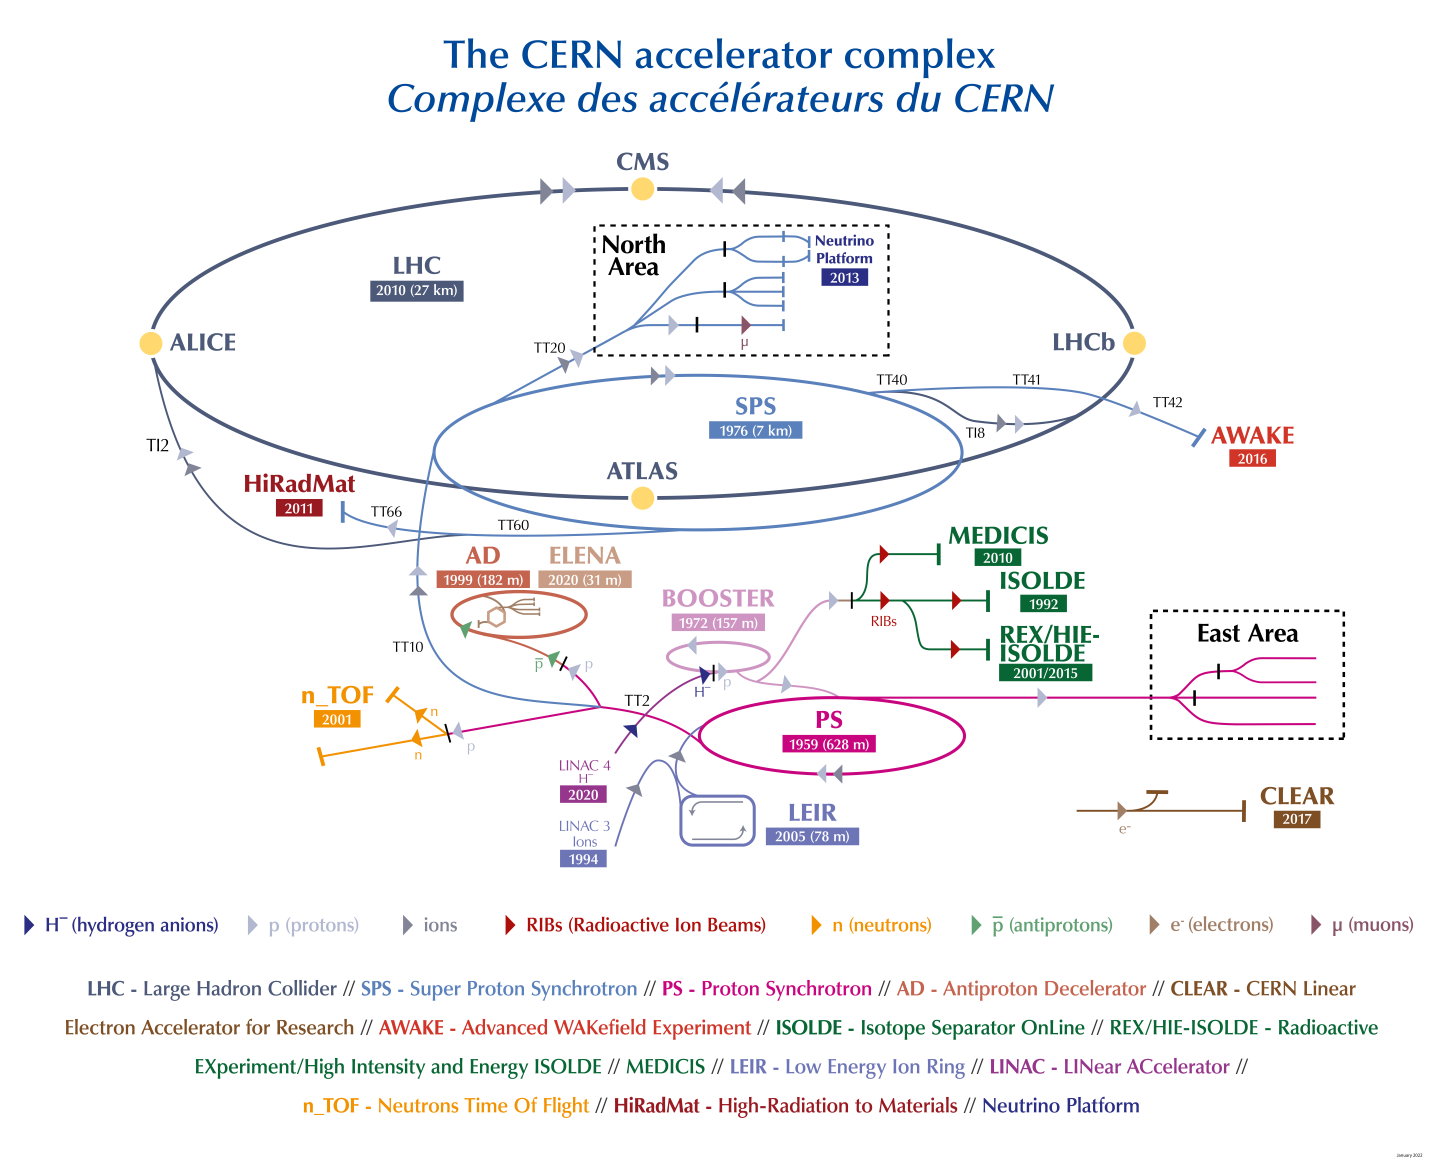
\includegraphics[width=\textwidth]{figures/CCC-v2022-large.png}
    \caption{The CERN accelerator complex is a succession of machines with increasingly higher energies. Each machine accelerates a beam of particles to a given energy before injecting the beam into the next machine in the chain. This next machine brings the beam to an even higher energy and so on. The LHC is the last element of this chain, in which the beams reach their highest energies.}
    \label{fig:LHC_scheme}
\end{figure}
The LHC operates with two beams of protons or lead ions circulating in opposite directions in separate beam pipes. The accelerator contains over 1200 superconducting dipole magnets, each about 15 metres long, to bend the beams, while 392 quadrupole magnets maintain beam focus. To ensure optimal performance, these magnets are cooled to \SI{1.9}{\kelvin} using superfluid helium. The high-energy beams collide at four designated points along the LHC ring, which house the major experiments: ATLAS, CMS, ALICE, and LHCb.

The experiments at the LHC serve different purposes. ATLAS and CMS are general-purpose detectors focusing on high-luminosity collisions to study a wide range of physics phenomena, including the search for new particles, extra dimensions, and dark matter. ALICE, a heavy-ion experiment, explores the quark-gluon plasma, a state of matter present shortly after the Big Bang. LHCb specializes in heavy-quark physics and operates at mid-range luminosity, focusing on flavor physics and $\mathcal{CP}$ violation studies.

Proton beams within the LHC are divided into 2808 bunches, each containing approximately $10^{11}$ protons. These bunches are time-spaced by multiples of \SI{25}{\nano\second}, resulting in a bunch-crossing frequency of up to \SI{40}{\mega\hertz}, with an average bunch-crossing rate of approximately \SI{30}{\mega\hertz}. 

The LHC has undergone significant upgrades during its operation. After LS2, which included improvements to the magnets and other critical systems, the LHC restarted with a center-of-mass energy of $\sqrt{s}=\SI{13}{\tera\eV}$, maintained throughout Run 2 (2015–2018). During Run 3, began in 2022, the LHC aimed to reach its peak design parameters, including a center-of-mass energy of $\sqrt{s}=\SI{14}{\tera\eV}$ and an instantaneous luminosity of $\mathcal{L}\approx\SI{2e34}{\per\centi\meter\squared\per\second}$.


\section{The LHCb Detector}

The LHCb detector depicted in Figure \ref{fig:lhcb-detector} is a single-arm forward spectrometer, with a pseudorapidity coverage of 2 to 5. This unique design allows it to study particles containing heavy quarks, primarily bottom (b) and charm (c), which are typically produced at high pseudorapidity during proton-proton (pp) collisions. The LHCb underwent a significant upgrade during LS2 to accommodate increased luminosity and handle the elevated event rate associated with the upgraded LHC.
\begin{figure}[h]
    \centering
    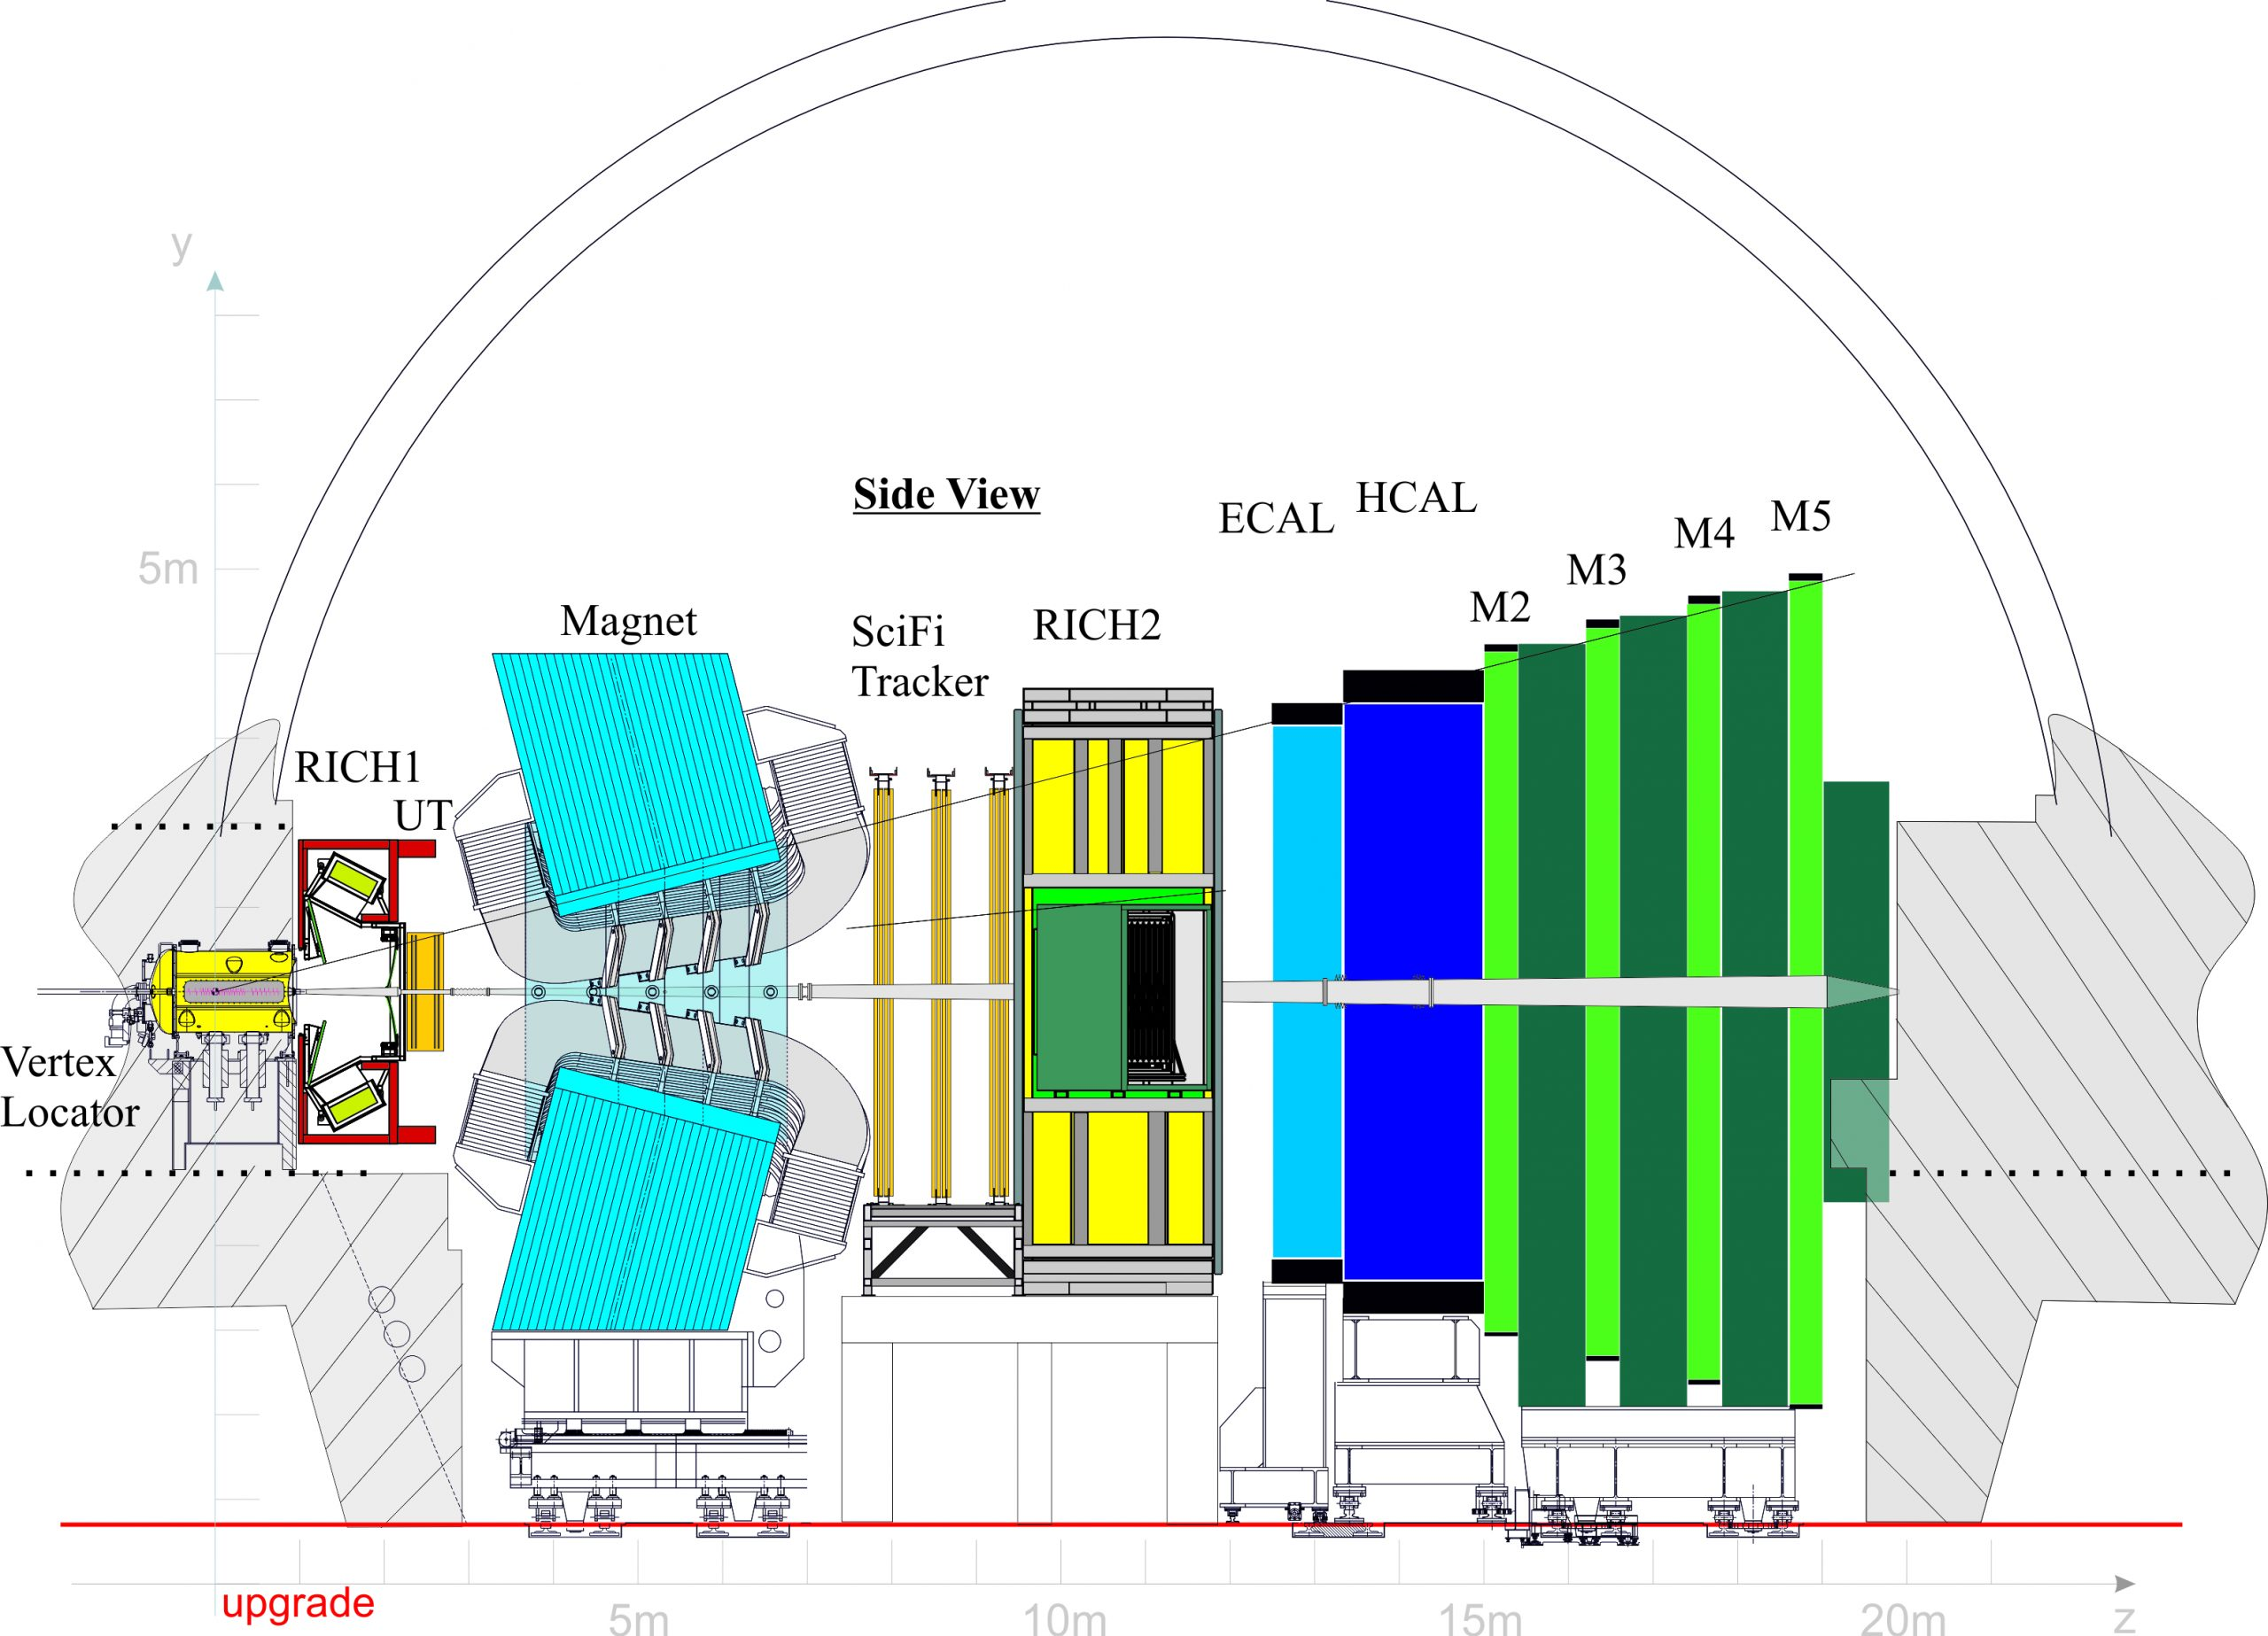
\includegraphics[width=\textwidth]{figures/UT-upgrade-detector-scaled.jpeg}
    \caption{Layout of LHCb-Upgrade I detector, side-view from the center of LHC ring.}
    \label{fig:lhcb-detector}
\end{figure}
With the upgrade, LHCb is expected to operate at an average bunch-crossing rate of approximately 30 MHz, with an expected instantaneous luminosity of about \SI{2e33}{\per\centi\meter\squared\per\second}. The average number of pp collisions per bunch-crossing is anticipated to be around 7.6. During Run-3 and Run-4, the experiment aims to collect at least \SI{50}{\per\femto\barn} of data, enabling unprecedented precision in measurements within the flavor sector of the Standard Model.

Key upgrades include:
\begin{itemize}
\item \textbf{Tracking System}: The tracking system has been revamped, with a new silicon detector, the Vertex Locator (VELO), which measures primary and secondary vertex positions with high precision. Additionally, there's a silicon strips upstream tracker (UT) and a scintillating fibers tracker (SciFi) for track fitting. A dipole magnet, generating a magnetic field with bending power of about 4 T·m, is placed between the UT and SciFi.

\item \textbf{Particle Identification}: The experiment uses two Cherenkov detectors, RICH1 (located before the UT) and RICH2 (after the SciFi), to identify charged hadrons. The Electromagnetic Calorimeter (ECAL) and Hadronic Calorimeter (HCAL) are used to detect electrons, photons, and hadrons, while the Muon Stations, located farthest from the interaction point, are dedicated to muon identification.

\item \textbf{Trigger System}: The trigger system has been completely overhauled. In previous runs, LHCb used a Level-zero (L0) hardware trigger, which reduced the bunch-crossing rate from 40 MHz to 1.1 MHz, based on information from the Calorimeter system and Muon stations. However, with increased luminosity, this system proved to be inefficient, leading to its removal. The upgraded trigger system now reconstructs the entire event data in real-time, enabling high selection efficiency for a wide range of events. The upgraded data acquisition system allows LHCb to process all the data from each collision in real-time, ensuring that no important events are missed. This system plays a crucial role in ensuring the experiment's ability to handle increased data flow and maintain high selection efficiency.
\end{itemize}
In the following sections an overview of each module of the detector will be given.

\subsection[VErtex LOcator]{VErtex LOcator $\bigl($VELO$\bigr)$}
The Vertex Locator (VELO)\cite{Bediaga:2013tje} is the innermost sub-detector of the LHCb experiment, designed to reconstruct primary and secondary decay vertices with high spatial resolution. This capability is critical for identifying displaced vertices of particles containing heavy quarks, such as charm and bottom hadrons, which have a decay length ranging from 100 to \SI{500}{\micro\meter}. At the trigger level, the VELO detects tracks with high impact parameters, which are indicative of heavy-flavored particle decays, helping reducing the minimum bias rate by providing initial track information. Offline, high-resolution vertex reconstruction is key to studying heavy-meson oscillations and CP-dependent time asymmetries.

The VELO is a silicon pixel detector designed to operate at high frequencies (up to 40 MHz) and withstand intense radiation levels. The detector is placed within the LHC vacuum pipe, allowing it to be positioned very close to the beamline. In its fully closed configuration, the innermost VELO sensor is just \SI{5.1}{\milli\meter} from the nominal interaction point, making it the closest detector to the beamline in any HEP experiment at CERN.
It consists of 26 stations, each made up of two halves (modules) surrounding the interaction point, both upstream and downstream. A brief schematics of the geometry is reported in Figure \ref{fig:velo-geometry}\cite{LHCbVelo:2019flq}.

Each module contains two tiles, and each tile has two sensors. Each sensor consists of 768 × 256 pixels, with a thickness of 200 µm. Sensors are mounted on both sides of the substrate, with different orientations for the upstream and downstream sensors. 

\begin{figure}
    \centering
    \begin{subfigure}{0.48\textwidth}
    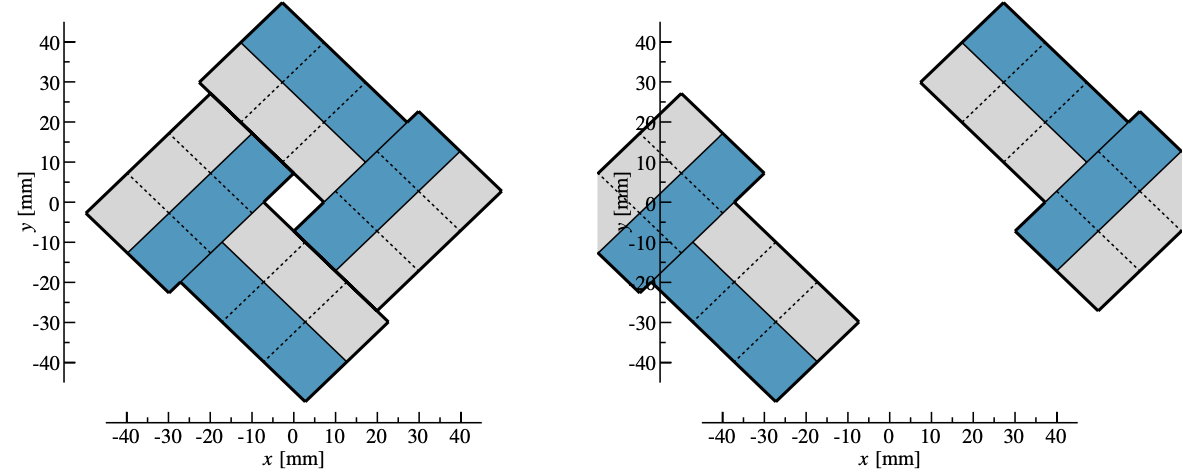
\includegraphics[width=\linewidth]{figures/aperture.png}
    \caption{XY view of a station (two modules: VELO A and VELO C)}\label{fig_velo-xy}
    \end{subfigure}
    \begin{subfigure}{0.48\textwidth}
    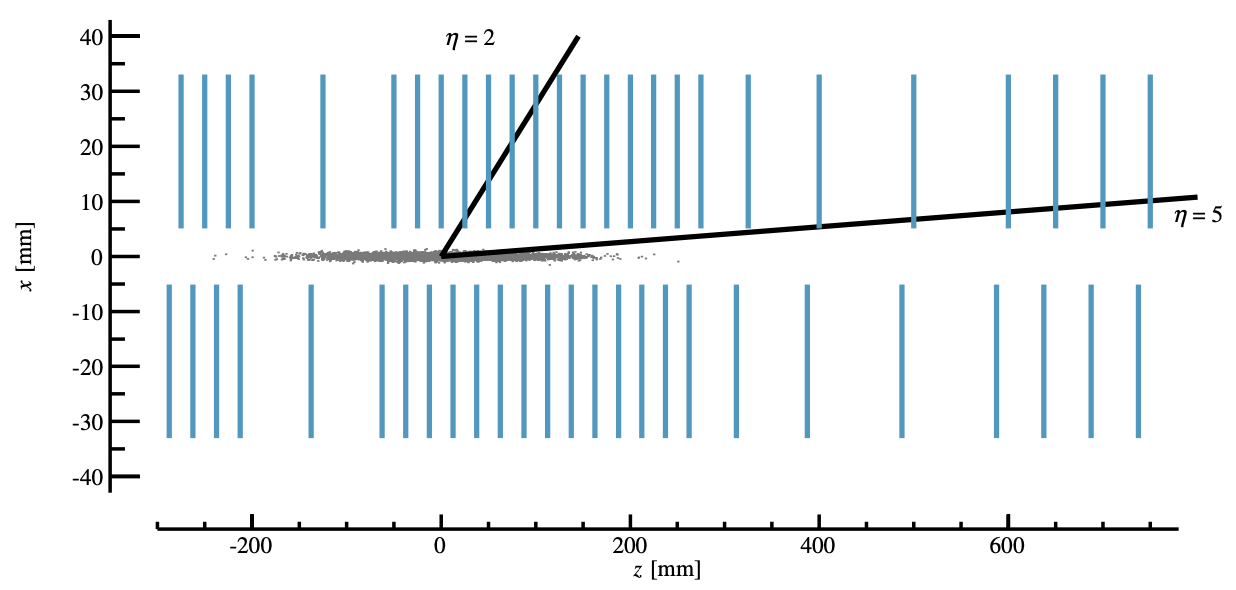
\includegraphics[width=\linewidth]{figures/above_view.png}
    \caption{Above view of all the 52 modules}\label{fig_velo-side}
    \end{subfigure}
    \caption{Two different schematics of the geometry of the VELO. Figure \ref{fig_velo-xy} shows a view of the plane perpendicular to the beampipe. The possible aperture of the two halves is also displayed. Figure \ref{fig_velo-side} shows a view from the side, where we appreciate each side section of the VELO.}
    \label{fig:velo-geometry}
\end{figure}

The VELO sensors are read out by VeloPix ASICs, each featuring a 256 × 256 matrix of active silicon pixels with dimensions of \SI{55}{\micro\meter} × \SI{55}{\micro\meter}. The entire VELO system contains over 40 million pixels. The raw hit resolution varies between 9 and \SI{15}{\micro\meter}, depending on the angle of the incoming particle. To maintain detection efficiency and account for highly inclined tracks, a 2-pixel wide overlap between sensors within the same tile is implemented. This overlap ensures no gaps in the detection coverage.
Due to the high-energy beams in the LHC, the VELO modules are not fixed in place during beam ramping to prevent damage from instabilities. During these periods, the modules are moved to a safer position, approximately 3 cm from the beamline, until the beams are stable.

\subsection{Upstream Tracker}
The UT is a micro-strip silicon detector made of four layers\cite{LHCb:2014uqj}. Each UT sensor is composed of \SI{250}{\micro\meter} thick silicon and a \SI{10}{\micro\meter} metalization layer. With near-beam sensor pitch of \SI{95}{\micro\meter} and dimension of 98×\SI{49}{\milli\meter}, it upgraded the old TT sensor pitch. In Figure \ref{fig:UT} a view of the detector is shown\cite{ut}. 
The UT is a core part of the LHCb physics case, being required to constrain important decays such as $K_S^\rightarrow\pi\pi$ that decay beyond the VELO acceptance. The UT also boosts the momentum resolution and helps identify ghost tracks.

\begin{figure}
    \centering
    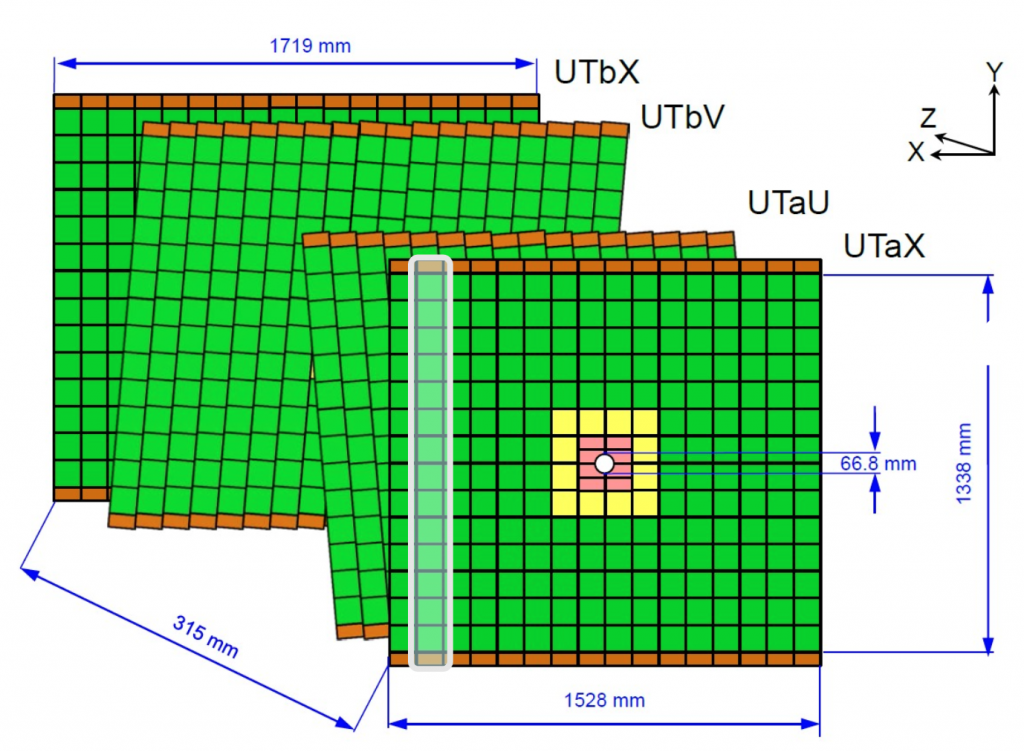
\includegraphics[width=0.8\textwidth]{figures/UT.png}
    \caption{Overview of the UT schematic layout.}
    \label{fig:UT}
\end{figure}

\subsection{Magnet}
LHCb exploits the forward region of proton collisions and requires a dipole field with a free aperture of ±300 mrad horizontally and ±250 mrad vertically. In order to achieve this, LHCb has magnet\cite{LHCb:2000xej} consisting of two coils, both weighing 27 tonnes, mounted inside a 1,450 tonne steel frame. Each coil is constructed from 10 ‘pancakes’, wound from almost 3,000 metres of aluminium cable. A schematics of the magnet is depicted in Figure \ref{fig:magnet}.
Tracking detectors in the magnetic field have to provide momentum measurement for charged particles with a precision of about 0.4\% for momenta up to 200 GeV/c. This demands an integrated field of 4 Tm for tracks originating near the primary interaction point.
A good field uniformity along the transverse co-ordinate is required by the muon trigger. The lateral aperture of the magnet is defined by the longitudinal extension of the detectors, placed upstream of the magnet. The magnet’s two coils are each 7.5 m long, 4.6 m wide and 2.5 m high.
\begin{figure}
    \centering
    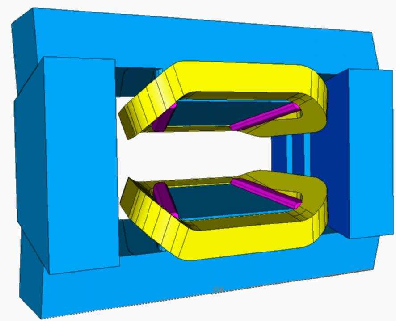
\includegraphics[width=0.6\textwidth]{figures/lhcb-magnet.png}
    \caption{A schematic of the LHCb Magnet}
    \label{fig:magnet}
\end{figure}
The LHCb magnet has a unique feature consisting into the possibility to reverse the polarity of the magnetic field (MagUp or MagDown). This allows a precise control of the charge asymmetries introduced by the detector. Particles hit preferentially one side of the detector, depending on their charges, generating large detection asymmetries. If data samples collected with the two different polarities have approximately equal size and the operating conditions are stable enough, effects of detection charge asymmetries are expected to cancel.

\subsection[Scintillating Fibre Tracker]{Scintillating Fibre Tracker$ \bigl($SciFi$\bigr)$}
The Scintillating Fibers tracker (SciFi)\cite{scifi} provides enhanced pattern recognition, momentum estimation, and overall tracking efficiency.
SciFi is located downstream of the dipole magnet and consists of three tracking stations: T1, T2, and T3. Each station comprises four detection planes, arranged to measure coordinates in a cross-pattern, with the orientation of the fiber strips at angles of 0°, +5°, -5°, and 0° relative to the vertical axis. This configuration offers high resolution in the bending plane of the magnetic field and supports efficient pattern recognition for charged particles.

The structural design features vertical staves in the first and last detection planes, while the central two have tilted staves, creating a balanced configuration that enhances detection capabilities and minimizes gaps in coverage. Each detector module is constructed with 2.5-meter-long scintillating fibers,\SI{250}{\micro\meter} in diameter. The modules closest to the beam pipe contain six fiber layers to manage higher radiation exposure, while the remaining modules, due to lower radiation levels, contain five layers.
A scheme of its geometry is reported in Figure \ref{fig:scifi}.
Scintillating fibers are made from a polymer core with 1\% by weight of fluorescent dye added to enhance scintillation. The fibers generate optical photons upon interaction with ionizing radiation. This process involves depositing energy in the polymer core, which excites the material. Due to the inherent limitations of the base polymer in terms of light yield and relaxation time, the addition of the fluorescent dye improves efficiency by matching energy-level structures to enhance photon production.

SciFi uses Silicon Photomultipliers (SiPMs) to read the optical photons. These SiPMs are contained in "Read-out Boxes" located at the top and bottom of each detection plane, ensuring efficient collection and processing of the scintillation signals. The SiPMs offer high gain, fast response, and compactness, allowing them to be integrated into the compact design of the SciFi system.

The SciFi system encompasses three stations, each consisting of four x−u−v−x layers. These layers are made up of 12 modules, measuring \SI{5}{\meter} by \SI{52}{\centi\meter}, with the innermost modules containing six fiber layers, and the others containing five. This design ensures high detection efficiency while keeping material within acceptable levels for reduced scattering and enhanced accuracy.

SciFi is designed for a high hit efficiency, with simulated performance indicating a hit efficiency of over 97\% at the end of its operational lifetime. The raw hit resolution is expected to be approximately 42 µm, providing precise measurements of charged particle trajectories.

The robustness of the SciFi system is further underscored by its ability to withstand the higher radiation levels experienced in the upgraded LHCb experiment, thanks to its optimized design and use of radiation-resistant materials. Its modular structure, with the Read-out Boxes, ensures easy maintenance and adaptability to evolving requirements.

\begin{figure}
    \centering
    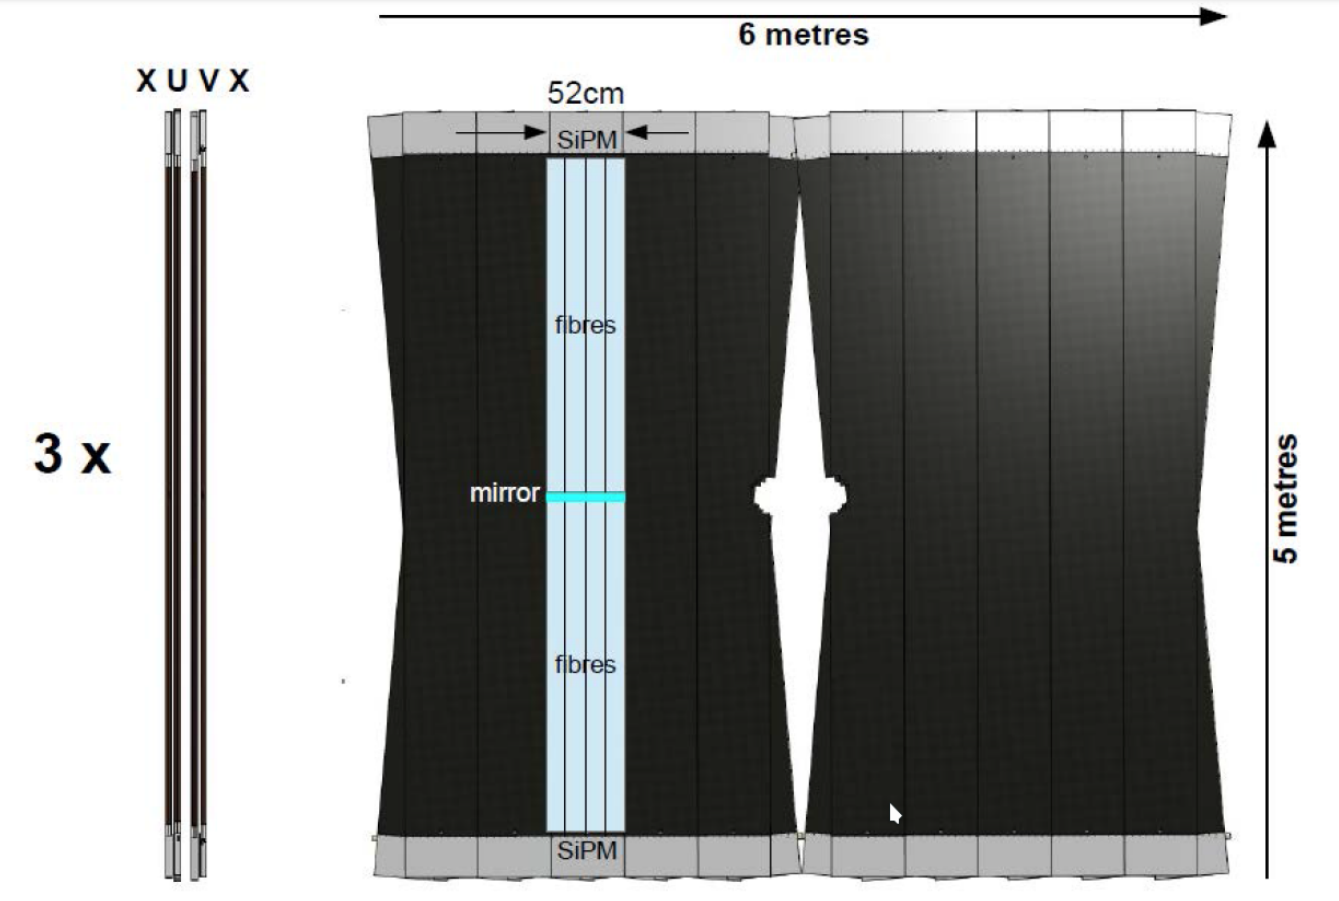
\includegraphics[width=\textwidth]{figures/scifi.png}
    \caption{A schematics of the SciFi}
    \label{fig:scifi}
\end{figure}


\subsection{RICH}
At LHCb there are two Ring Imaging Cherenkov (RICH) detectors, RICH1 and RICH2, that enable particle identification\cite{LHCb:2013urp} across a broad momentum range, from 1 to 100 GeV/c\cite{Adinolfi_2013}.

Cherenkov radiation occurs when charged particles travel through a dielectric medium at speeds exceeding the local speed of light (superluminal speed). The angle at which Cherenkov radiation is emitted (Cherenkov angle) is directly related to the refractive index of the medium and the velocity of the particle. Given this relation, the Cherenkov angle, θc, can be used to infer the mass of a particle when its momentum is known:

\begin{equation}
    \cos\theta_c=\frac{1}{\beta n} = \frac{1}{n}\sqrt{1+\biggl(\frac{m}{p}\biggr)^2}
\end{equation}

where $\beta$ is the speed of the particle relative to the speed of light, $n$ is the refractive index of the medium, $m$ is the particle's mass, $p$ is its momentum.
This principle allows for the identification of different particles based on the Cherenkov angle. The RICH system uses this concept to separate charged hadrons over a momentum range of 1–100 GeV/c, essential for studying hadronic final states and central to LHCb's physics goals, including precise measurements of $\mathcal{CP}$ violation and rare decays of b and c hadrons.

RICH1 is located between the VELO and the UT, upstream of the spectrometer magnet. It uses two radiators, aerogel (with refractive index $n=1.03$) and C4F10 (with refractive index $n=1.0014$), allowing discrimination of particles over a momentum range of 1–60 GeV/c. RICH1 covers an angular acceptance of 25–300 mrad.

RICH2 is downstream of the spectrometer magnet, after the last T-station, covering an angular acceptance from 15 to 120 (non-bending plane) and 15 to 100 mrad (bending plane). It uses CF4 (with refractive index $n=1.0005$) as the radiator, allowing discrimination of particles with momentum ranging from 15 to ≥100 GeV/c. The π−K separation in RICH2 is approximately 90\% efficient for momenta up to 30 GeV/c.

The RICH detectors use spherical mirrors to focus Cherenkov light, with secondary flat mirrors to guide the photons onto Hybrid Photon Detectors (HPDs). These HPDs are sensitive to photons in the 200–600 nm wavelength range and are placed outside the detector acceptance, reducing material costs and protecting them from the spectrometer's magnetic field.

Arrays of 'multi-anode photomultiplier tubes' (MaPMTs) are used to detect individual Cherenkov photons, with RICH1 having a total detection area of 1.6 m² and RICH2 having a detection area of 2.1 m². This arrangement ensures efficient collection and processing of Cherenkov light for particle identification.

\begin{figure}
    \centering
    \begin{subfigure}{0.48\textwidth}
    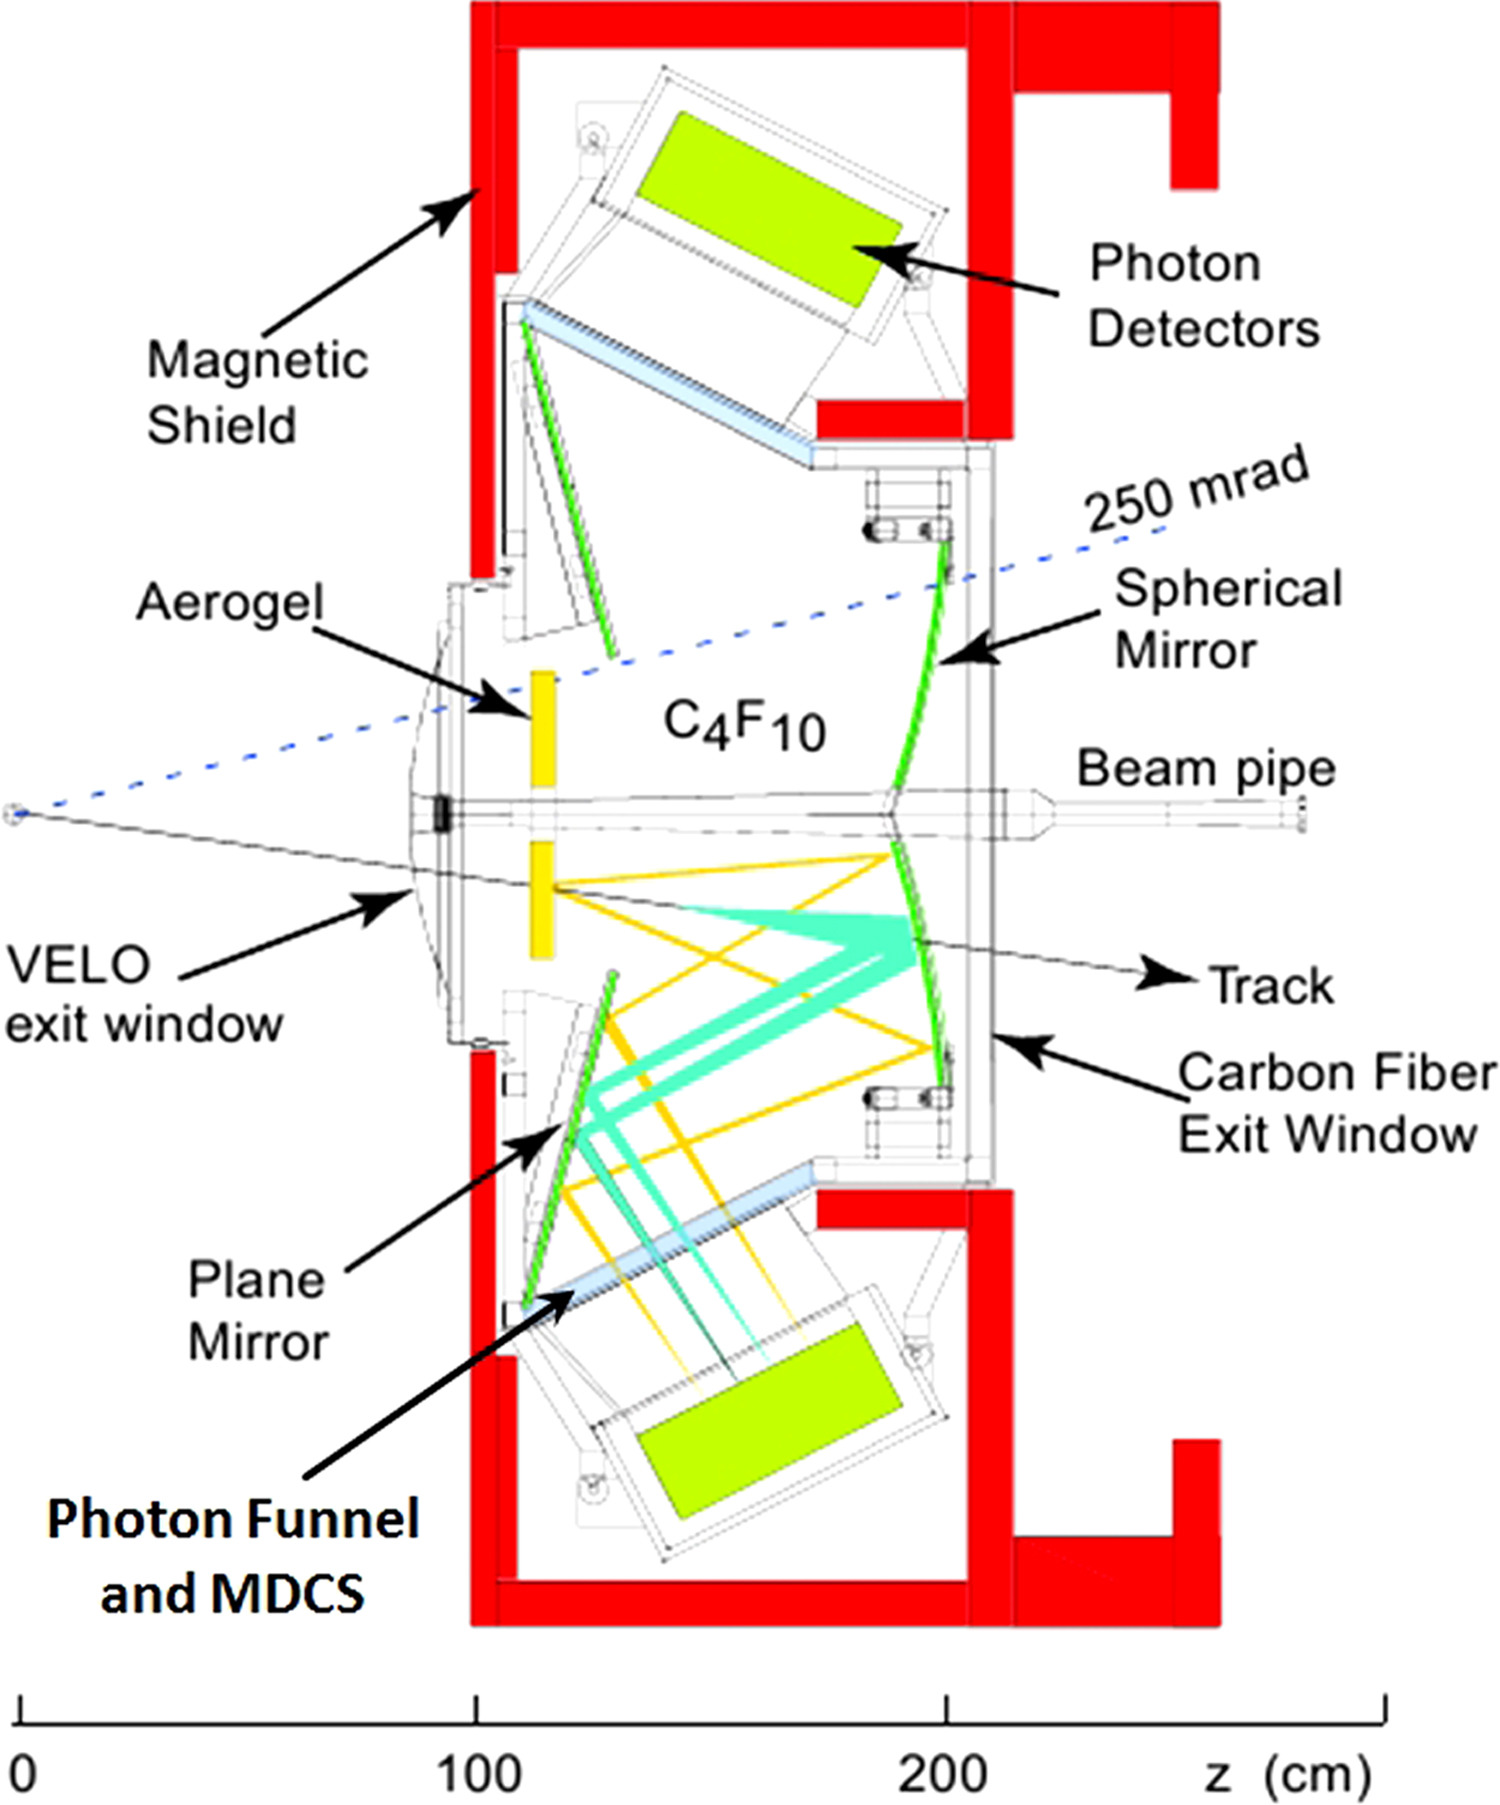
\includegraphics[width=\linewidth]{figures/rich1.jpg}
    \caption{RICH1}\label{RICH1}
    \end{subfigure}
    \hfill
    \begin{subfigure}{0.48\textwidth}
    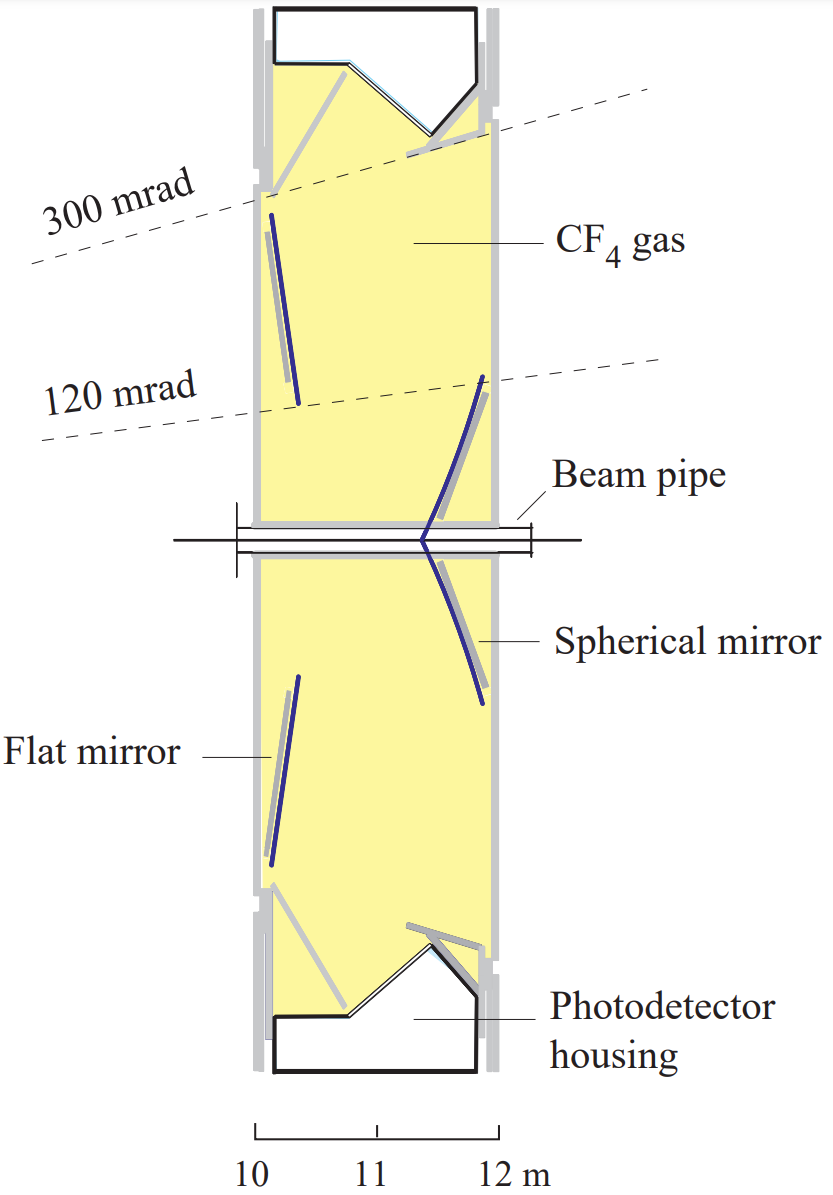
\includegraphics[width=0.78\linewidth]{figures/rich2.png}
    \caption{RICH2}\label{rich2}
    \end{subfigure}
    \caption{Schematics side view of the two RICH detectors.}
    \label{fig:rich}
\end{figure}

\subsection{Calorimeters}
The calorimeter system in the LHCb experiment\cite{LHCb:2000vji} plays its role in identifying electrons, photons, and hadrons, providing a raw measurement of their energies and positions. The system comprises the Electromagnetic Calorimeter (ECAL) and an  Hadron Calorimeter (HCAL). Both of them are  placed between the first and second muon stations, with an angular acceptance ranging from 25 mrad to 300(250)mrad in the bending (non-bending) plane. 
The ECAL is responsible for measuring the energy and position of electrons and photons. It is built with shashlik calorimeter technology, consisting of alternating 4 mm-thick polystyrene scintillating tiles and 2 mm lead sheets. The scintillation light is collected using wavelength-shifting fibers and read out by individual photomultipliers (PMTs) mounted at the back of the tiles. The total thickness of the ECAL is 25 radiation lengths, providing sufficient thickness to contain most electromagnetic showers. The calorimeter structure is segmented into three zones depending on the radial distance from the beamline. The inner section has cells with a lateral dimension of 40.4 mm, the middle section has cells with a 60.6 mm dimension, and the outer section comprises cells with a 121.2 mm dimension. The energy resolution for the ECAL is approximately 
 $\sigma_E/E$(GeV)=(8.5−9.5).

The HCAL is responsible for measuring the energy and position of hadrons. It consists of 16 mm-thick iron layers alternated with 2 mm scintillating fibers, with a total thickness corresponding to 5.6 nuclear interaction lengths. This design is constrained by the space available inside the LHCb cavern. The energy resolution for the HCAL is approximately $\sigma_E/E$(GeV)=(8.5−9.5)/E(GeV)=9. 
\subsection{Muon Stations}
The muon detector system's primary function is to identify and measure the transverse momentum of muons in order to reconstruct decay channels involving muons, which are vital for many LHCb physics studies.
The LHCb muon detector system\cite{Alves_2013} consists of four stations (M2 to M5) placed downstream of the hadronic calorimeter and interleaved with thick iron walls that act as muon filters. In Run-1 and Run-2, there was an additional M1 station located in front of the calorimeters, used for transverse momentum measurement for the L0 trigger\cite{muon_upgrade}. The system covers the angular acceptance from 20 (16) to 306 (258) mrad in the bending (non-bending) plane. Each station comprises two mechanically independent halves, called the A and C sides, which can be horizontally moved to access the beam pipe and detector chambers for installation and maintenance.
A scheme of the muon stations (including M1 no longer part of the detector) is depicted in Figure \ref{fig:muon}.
The stations are equipped with Multi-Wire Proportional Chambers (MWPCs) for muon detection. These chambers use a gas mixture of argon, carbon dioxide, and tetrafluoromethane (CF4) in varying proportions for optimal muon detection and signal collection. The iron absorbers between the stations add to the muon filtering capacity, ensuring that only muons with momentum greater than 6 GeV/c can traverse the entire system.

Stations M2-M3 focus on transverse momentum measurements, while M4 and M5 serve to confirm if a particle has traversed the entire detector system. The system achieves a 95\% detection efficiency, providing robust muon identification. 

The unique feature of the LHCb muon detector system is its segmented structure, with each station divided into four regions (R1-R4), with cells scaling in the ratio 1:2:4:8 with distance from the beam axis. This segmentation allows the system to manage varying particle rates and optimize detection efficiency. Additionally, the independent halves (A and C sides) offer flexibility during installation and maintenance, enabling quick access to the beam pipe and detector chambers when needed.
\begin{figure}
    \centering
    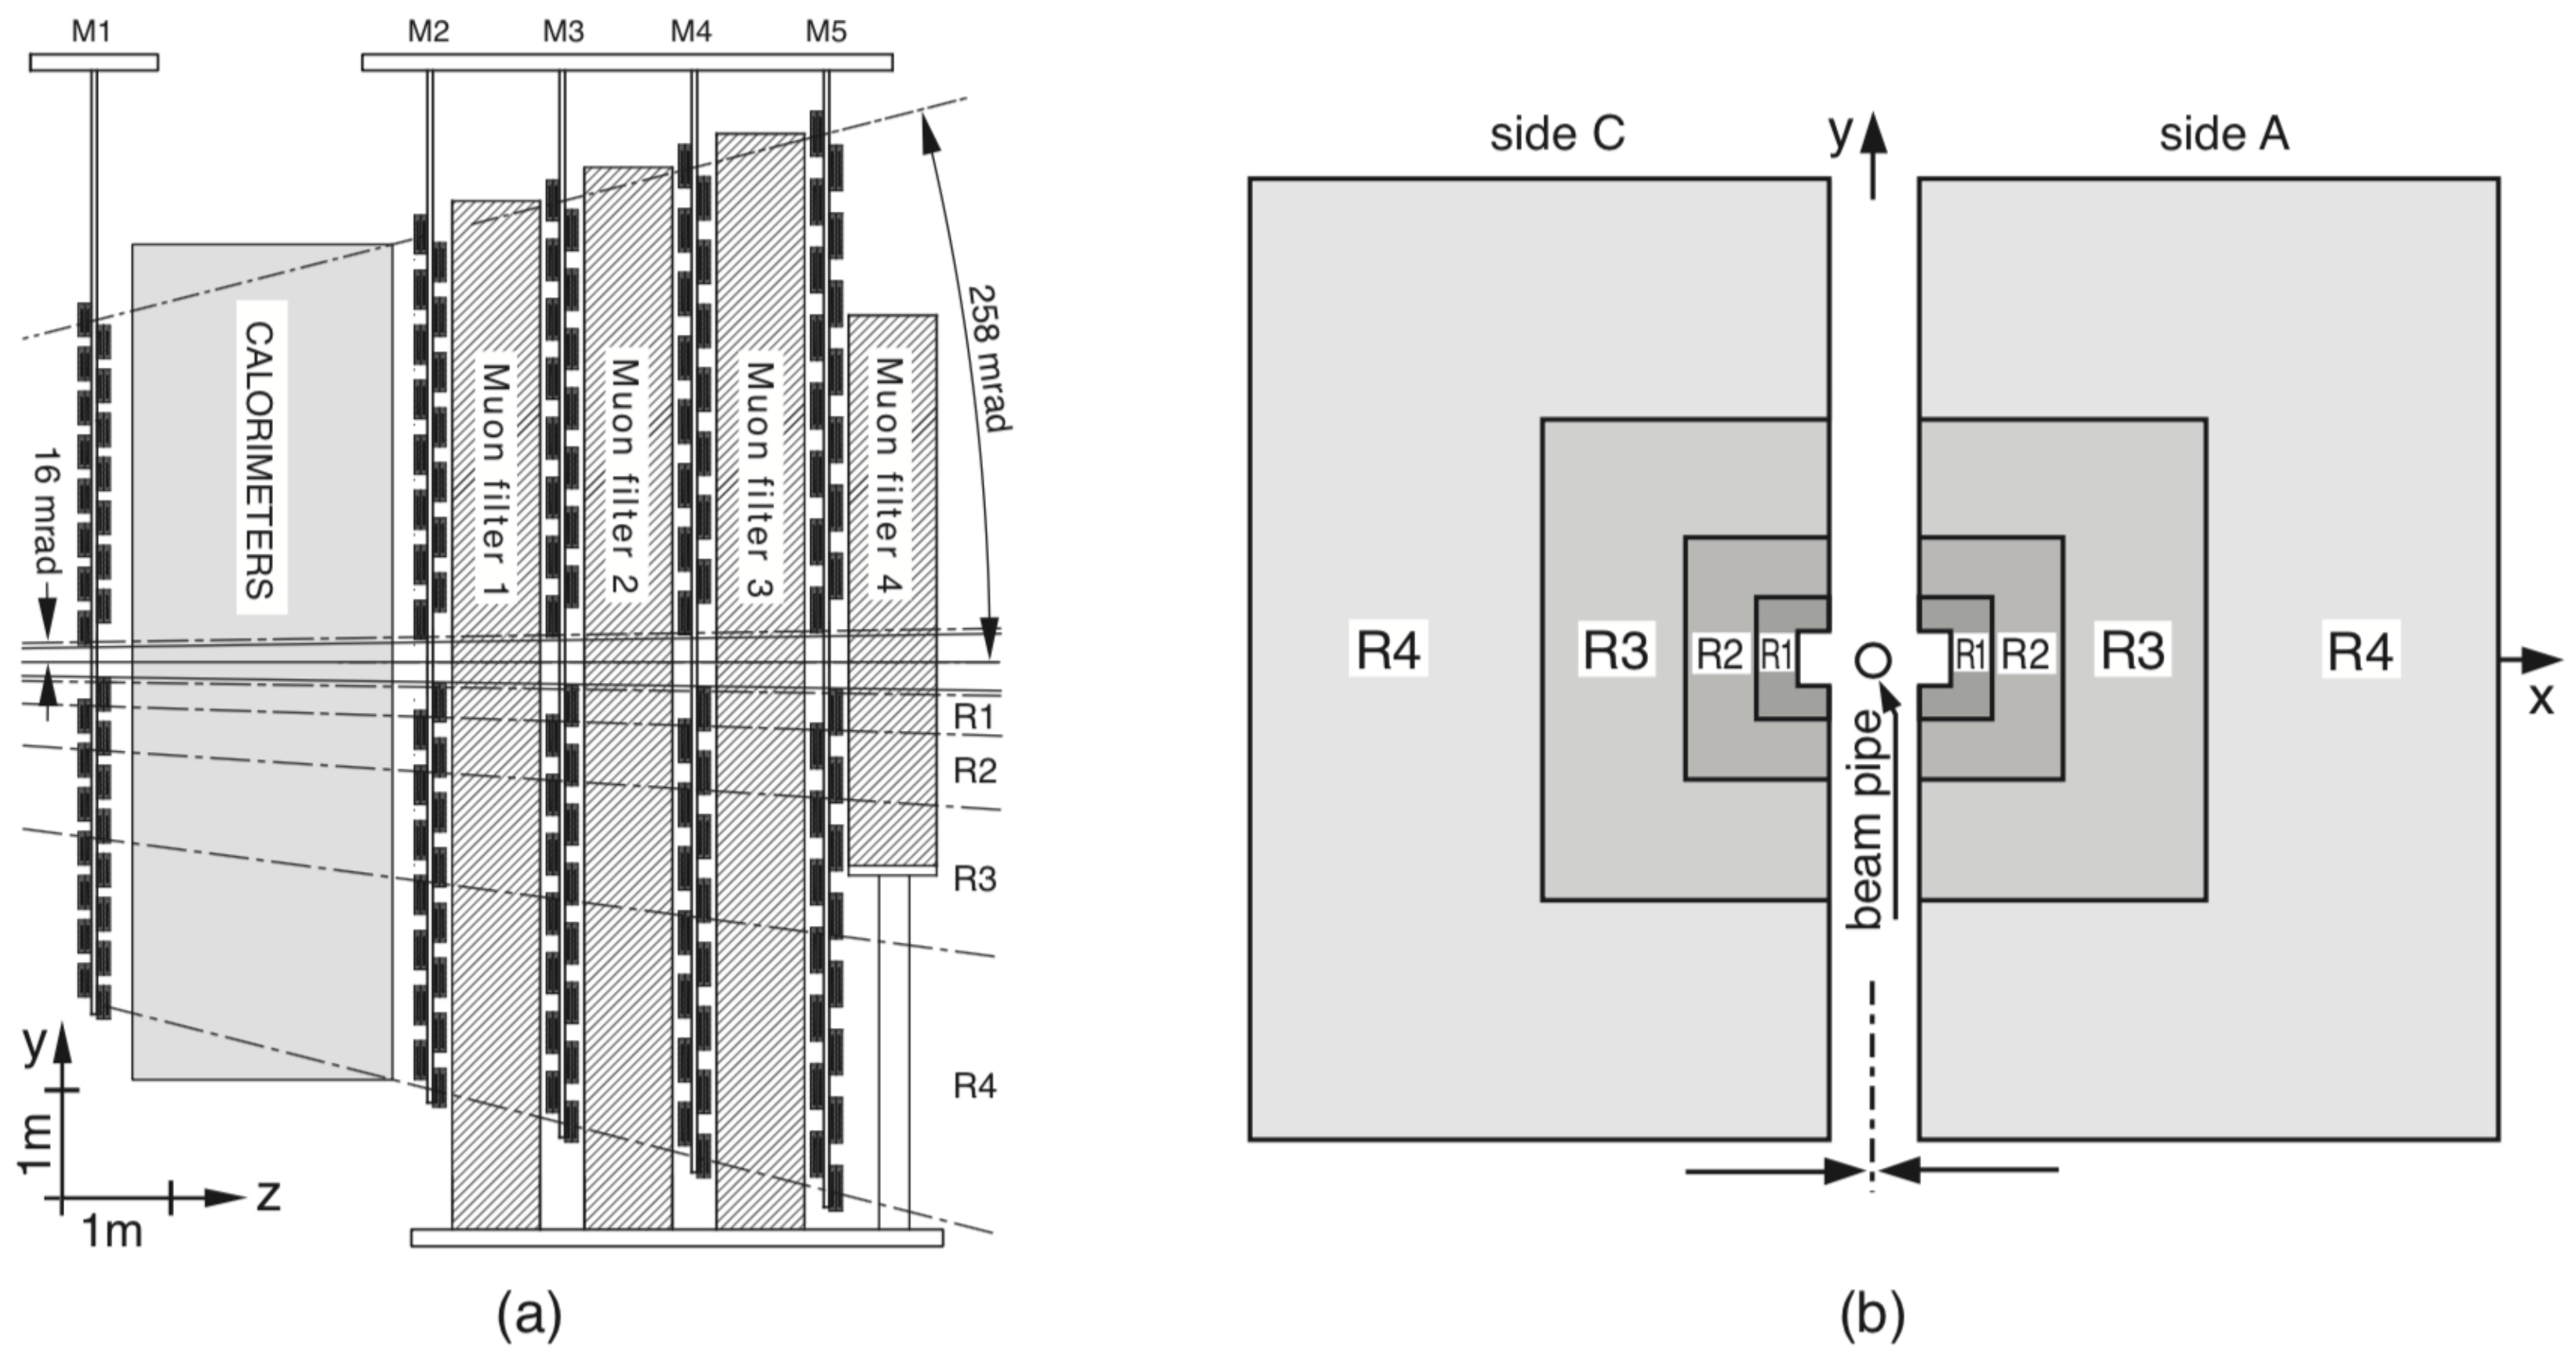
\includegraphics[width=\textwidth]{figures/muon.png}
    \caption{A scheme of the muon stations. M1 was removed during Upgrade 1.}
    \label{fig:muon}
\end{figure}

\section{Real Time Analysis}\label{sec:rta}
\begin{figure}
    \centering
    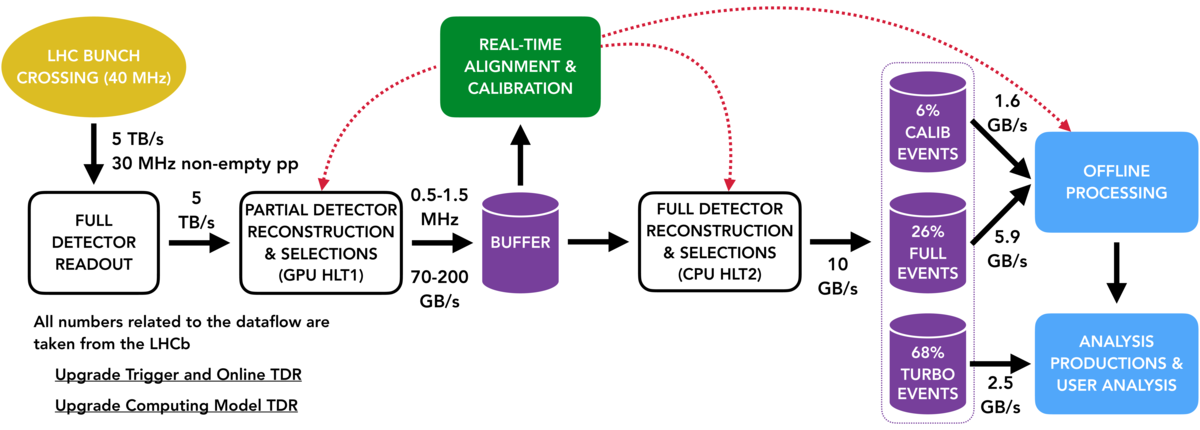
\includegraphics[width=\textwidth]{figures/hidef_RTA_dataflow_widescreen.png}
    \caption{Workflow of the RTA paradigm, from the detector readout to analysis production}
    \label{fig:RTA}
\end{figure}
With the increase in instantaneous luminosity at the LHCb interaction point, the demand for more accurate measurements has driven the collaboration to completely renew its readout and trigger systems. The upgraded system operates at an average event rate of 30 MHz, processing every event with a fully software-based trigger system that integrates information from all sub-detectors. The need for more efficient trigger systems emerged from simulation studies showing that the trigger sequence used during Run-1 and Run-2 would lead to a loss of efficiency in hadronic B-meson decay channels as the instantaneous luminosity increased\cite{CERN-LHCC-2011-001}. The first stage of the previous trigger system, L0, relied on transverse energy $E_T$ measurements from several sub-detectors, including charged hadrons, muons, electrons, or photons. This resulted in high efficiencies for dimuon events but reduced efficiency for fully hadronic signal decays. Additionally, the increase in the $E_T$ threshold to manage trigger rates with higher luminosities compromised signal efficiency in hadronic channels, causing saturation of the trigger yield.

The revamped DAQ and trigger system at LHCb is designed to overcome these limitations\cite{CERN-LHCC-2018-014}. The new system operates at full LHC bunch crossing rate, with event reconstruction based on precise measurements of momentum and impact parameters. The readout system can handle high input data flow, on the order of 50 TB/s, while the software-based trigger can process data at an average rate of 30 MHz.

The trigger system now implements a two-stage full software solution:
\begin{itemize}
\item HLT1: The first stage, implemented on Graphics Processing Units (GPUs), operates on Event Builder (EB) nodes, reducing the data rate by a factor of 30-60.
\item HLT2: The second stage, running on Central Processing Units (CPUs) allows for detailed event reconstruction with quasi-offline precision\cite{Gazzoni:2670650}.
\end{itemize}
Between HLT1 and HLT2, a buffer is implemented where the Alignment \& Calibration phase of the detector elements is performed.

The DAQ system\cite{CERN-LHCC-2014-016} is composed of several sub-systems:
\begin{itemize}
\item Event Builder (EB)
\item Timing and Fast Control (TFC)
\item Event Filter Farm (EFF)
\item Experimental Control System (ECS)
\end{itemize}
In the following subsections, an overview of each subsystem is going to be presented. 

\subsection{Event Builder}
The data from all the sub-detectors in the underground area are transmitted to the surface through radiation-hard 300-meter-long optical fibers with zero-suppression, reducing unnecessary information before being transmitted. Each detector sends its data to a specific set of EB nodes. Within each EB node, custom PCIe boards (called PCIe40) equipped with FPGA chips process the incoming data, providing an interface between the front-end electronics and the other control systems, such as TFC and ECS). This preprocessing step is crucial, as it reduces the data load for subsequent stages. Each EB node processes a portion of the event data, requiring to exchange information with other EB nodes to assemble complete event information. This distributed approach reduces the amount of data any single node must process, ensuring efficiency and scalability. The EB nodes are interconnected through the Event Builder Network, which is designed to facilitate high-speed data exchange and event building.




\subsection{Timing and Fast Control}
The TFC system is responsible for distributing critical clock, timing, and trigger information to the front-end and readout systems. It synchronizes to the LHC master clock, ensuring precise timing across all components. The TFC provides global signals, including the 40 MHz clock, synchronous commands to control event processing, calibration commands for detectors, and electronics configuration distribution from the ECS.

\subsection{Event Filter Farm}
The Event Filter Farm (EFF) hosts the hardware architectures for the high-level triggers (HLT). The HLT sequence comprises two stages: HLT1 and HLT2, separated by a disk buffer that holds events between stages while the detector is aligned and calibrated with offline precision.
\subsubsection{HLT1}
The HLT1 stage aims to reject events that don't contain particles of interest while retaining those that do. It uses a subset of the full offline charged particle reconstruction and implements inclusive single or two-track selections to determine the event's interest. HLT1 is entirely implemented on GPUs in the same servers hosting the Event Builder. The \textit{Allen} application, written in C++ with CUDA extensions, executes the following tasks\cite{CERN-LHCC-2020-006}:
\begin{itemize}
\item Decoding raw input into the LHCb global coordinate system
\item Clustering detector hits
\item Pattern recognition to identify hit combinations associated with the same particle
\item Fitting track candidates using a Kalman Filter to estimate momentum and other parameters
\item Reconstructing primary and secondary vertices from fitted tracks
\item Making trigger decisions based on track parameters like impact parameter and momentum
\end{itemize}
\subsubsection{Alignment and Calibration}\label{sec:alignment}
LHCb distinguishes between two phases\cite{Dziurda:2640712}:
\begin{itemize}
\item Alignment focuses on correcting shifts and rotations in the detector's components, ensuring that the data obtained from these detectors are accurate. This process is applied to tracking detectors like VELO, UT, SciFi, and Muon systems, ensuring that their positioning aligns with the expected geometry.
\item Calibration involves fine-tuning the responses of various sub-detectors to ensure accurate measurements. This includes calibrating the RICH, ECAL, and HCAL.
\end{itemize}
Both processes are triggered at the beginning of each LHC fill, and they are fully integrated into the LHCb control system. 
\paragraph{Alignment}
Alignment at LHCb involves minimizing the chi-squared $\chi^2$ of all tracks with respect to alignment parameters $\alpha$, which account for translations and rotations of detector elements. The procedure employs the iterative Newton-Raphson method, where the first and second derivatives of $\chi^2$ with respect to 
 $\alpha$ are calculated to determine the optimal adjustments needed for alignment. The data for this alignment procedure comes from tracks obtained through a Kalman filter used in track reconstruction\cite{HULSBERGEN2009471}, with the option to add vertex and mass constraints for increased precision.

The alignment process has two key components\cite{Saur:20230E}:
\begin{itemize}
\item Analyzer: This part runs the track reconstruction, computes the $\chi^2$ derivatives, and saves them to binary files. It uses multi-threaded reconstruction based on 163 nodes, allowing for efficient data processing.
\item Iterator: This component collects the derivatives from the Analyzer, performs the minimization step, and checks for convergence. If there is a significant difference between the previous and new alignment constants, the updated constants are used in the HLT2 trigger, ensuring that subsequent data collection reflects the corrected alignment.
\end{itemize}
\paragraph{Calibration}
Calibration at LHCb involves ensuring that the detector responses are accurate and consistent. It typically includes:
\begin{itemize}
\item RICH Calibration: This involves calibrating the mirror positions and alignment to ensure accurate Cherenkov angle measurements.
\item Calorimeter Calibration: ECAL and HCAL calibration focuses on ensuring accurate energy measurements.
\end{itemize}
The calibration process leverages dedicated HLT1 trigger lines to select events suitable for calibration and alignment. These events are stored in a buffer until sufficient statistics are accumulated to run the calibration and alignment procedure. This buffering allows HLT2 reconstruction to use the most accurate and relevant alignment and calibration constants.
\subsubsection{HLT2}
While HLT1 focuses on long tracks, HLT2 conducts a full reconstruction, using information from tracking detectors and particle identification systems (RICHs, calorimeters, and muon chambers). It applies specialized cuts to select events of interest to LHCb.

\subsection{Experimental Control System}
\textit{Description of ECS with a focus on WinCC.
}
The ECS\cite{GranadoCardoso:2702137} oversees the entire LHCb experiment, from infrastructure to data acquisition. It is a distributed system based on the commercial SCADA system, WinCC OA, and custom-developed components. The ECS features user interfaces, data archiving, alarm handling, and various device interfaces. Its tree-like control hierarchy, based on a Finite State Machine (FSM), allows commands to be propagated downstream and state information to be propagated upward. This structure provides centralized control and monitoring, ensuring efficient management of the LHCb experiment.
The majority of tracks are created near the interaction point, and these are reconstructed as long tracks. However, some neutral long-lived particles, like $K^0_S$ and $\Lambda^0$, are reconstructed as downstream tracks because they decay outside the acceptance of the VELO detector. HLT1 focuses on long tracks, while HLT2 includes downstream tracks in its reconstruction sequence, allowing more comprehensive event analysis.


%Example of \autoref{alg:1} reference.

%\begin{algorithm}
%    \caption{Pseudocode}
%    \label{alg:1}
%    \begin{algorithmic}
%        \STATE $i\gets 10$
%        \IF {$i\geq 5$} 
%          \STATE $i\gets i-1$
%        \ELSE
%          \IF {$i\leq 3$}
%            \STATE $i\gets i+2$
%          \ENDIF
%        \ENDIF 
%    \end{algorithmic}
%\end{algorithm}